\begin{figure}
  \centering 
  \begin{subfigure}[b]{0.45\textwidth}
    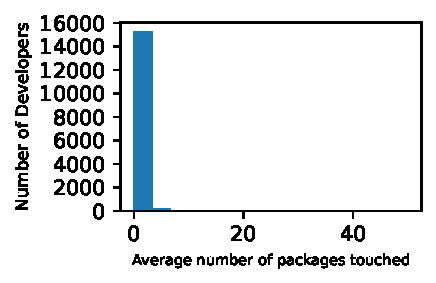
\includegraphics[width=\textwidth]{sections/results/graph/normality_and_homoscedasticity_graph_transient_moderate_1_packages_founder_transient.packages.touched.commits.pdf}
    \caption{Transient ($\mu$: 1.15, median:1.0, mode:1, std:0.92 and max:50)}
    \label{subfig:sections/results/graph/normality_and_homoscedasticity_graph_transient_moderate_1_packages_founder_transient_packages_touched_commits_pdf}
  \end{subfigure}
  \begin{subfigure}[b]{0.45\textwidth}
    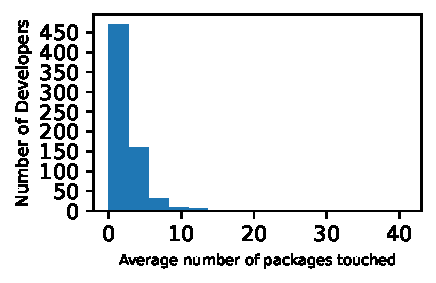
\includegraphics[width=\textwidth]{sections/results/graph/normality_and_homoscedasticity_graph_transient_moderate_1_packages_sample_moderate.packages.touched.commits.pdf}
    \caption{Moderate ($\mu$: 2.59, median:2, mode:1, std:3.06 and max:41)}
    \label{subfig:sections/results/graph/normality_and_homoscedasticity_graph_transient_moderate_1_packages_sample_moderate_packages_touched_commits_pdf}
  \end{subfigure}
\vspace{3mm}
  \begin{subfigure}[b]{0.45\textwidth}
    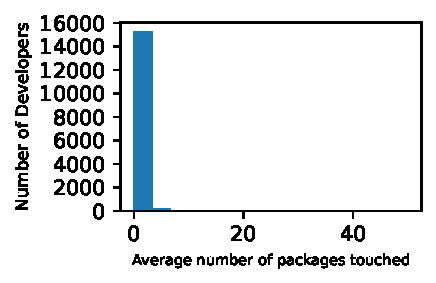
\includegraphics[width=\textwidth]{sections/results/graph/normality_and_homoscedasticity_graph_transient_moderate_1_packages_founder_transient.packages.touched.commits.pdf}
    \caption{Transient ($\mu$: 1.15, median:1.0, mode:1, std:0.92 and max:50)}
    \label{subfig:sections/results/graph/normality_and_homoscedasticity_graph_transient_moderate_1_packages_founder_transient_packages_touched_commits_pdf}
  \end{subfigure}
  \begin{subfigure}[b]{0.45\textwidth}
    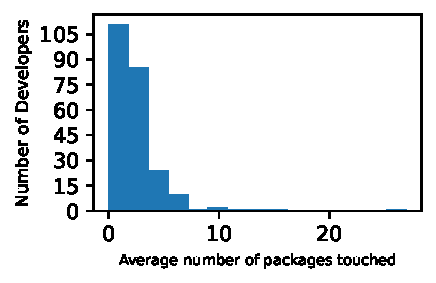
\includegraphics[width=\textwidth]{sections/results/graph/normality_and_homoscedasticity_graph_transient_moderate_1_packages_sample_sustained.packages.touched.commits.pdf}
    \caption{Sustained ($\mu$: 2.38, median:2, mode:1, std:2.61 and max:27)}
    \label{subfig:sections/results/graph/normality_and_homoscedasticity_graph_transient_moderate_1_packages_sample_sustained_packages_touched_commits_pdf}
  \end{subfigure}
\vspace{3mm}
  \begin{subfigure}[b]{0.45\textwidth}
    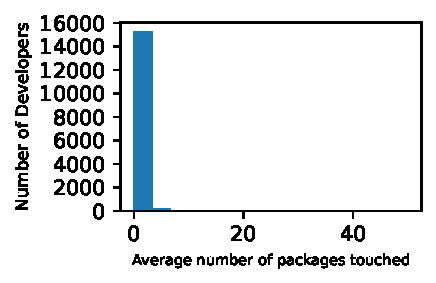
\includegraphics[width=\textwidth]{sections/results/graph/normality_and_homoscedasticity_graph_transient_moderate_1_packages_founder_transient.packages.touched.commits.pdf}
    \caption{Transient ($\mu$: 1.15, median:1.0, mode:1, std:0.92 and max:50)}
    \label{subfig:sections/results/graph/normality_and_homoscedasticity_graph_transient_moderate_1_packages_founder_transient_packages_touched_commits_pdf}
  \end{subfigure}
  \begin{subfigure}[b]{0.45\textwidth}
    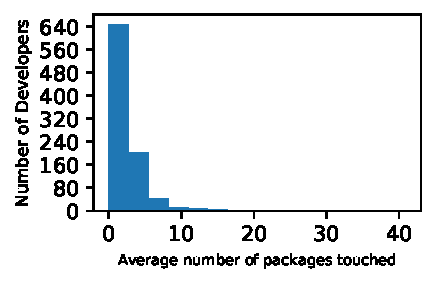
\includegraphics[width=\textwidth]{sections/results/graph/normality_and_homoscedasticity_graph_transient_moderate_1_packages_sample_moderate sustained.packages.touched.commits.pdf}
    \caption{Moderate sustained ($\mu$: 2.54, median:2.0, mode:1, std:2.95 and max:41)}
    \label{subfig:sections/results/graph/normality_and_homoscedasticity_graph_transient_moderate_1_packages_sample_moderate sustained_packages_touched_commits_pdf}
  \end{subfigure}
\vspace{3mm}
  \begin{subfigure}[b]{0.45\textwidth}
    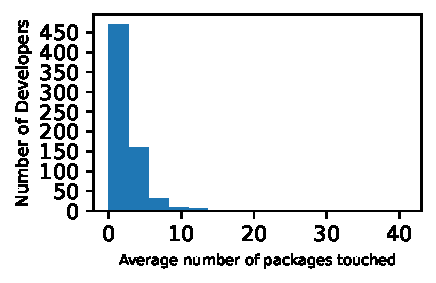
\includegraphics[width=\textwidth]{sections/results/graph/normality_and_homoscedasticity_graph_transient_moderate_1_packages_founder_moderate.packages.touched.commits.pdf}
    \caption{Moderate ($\mu$: 2.59, median:2, mode:1, std:3.06 and max:41)}
    \label{subfig:sections/results/graph/normality_and_homoscedasticity_graph_transient_moderate_1_packages_founder_moderate_packages_touched_commits_pdf}
  \end{subfigure}
  \begin{subfigure}[b]{0.45\textwidth}
    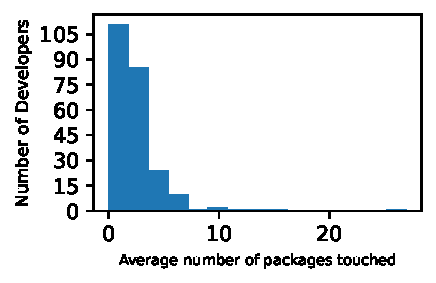
\includegraphics[width=\textwidth]{sections/results/graph/normality_and_homoscedasticity_graph_transient_moderate_1_packages_sample_sustained.packages.touched.commits.pdf}
    \caption{Sustained ($\mu$: 2.38, median:2, mode:1, std:2.61 and max:27)}
    \label{subfig:sections/results/graph/normality_and_homoscedasticity_graph_transient_moderate_1_packages_sample_sustained_packages_touched_commits_pdf}
  \end{subfigure}
\caption{Packages for one commits for  sample A category versus sample B category } 
    \label{fig:codebase_graph_latex_repository_graph_component_time_series_statistical_significance_testpackages1normality_and_homoscedasticity_graph_transient_moderate}
\end{figure}
\clearpage 
\begin{figure}
  \centering 
\vspace{3mm}
  \begin{subfigure}[b]{0.45\textwidth}
    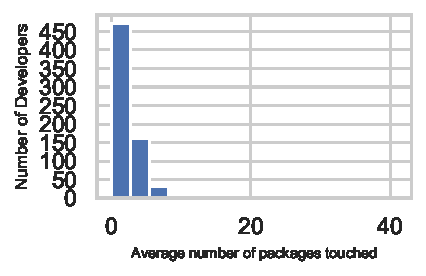
\includegraphics[width=\textwidth]{sections/results/graph/normality_and_homoscedasticity_graph_transient_moderate_2_packages_founder_moderate.packages.touched.commits.pdf}
    \caption{Moderate ($\mu$: 2.59, median:2, mode:1, std:3.06 and max:41)}
    \label{subfig:sections/results/graph/normality_and_homoscedasticity_graph_transient_moderate_2_packages_founder_moderate_packages_touched_commits_pdf}
  \end{subfigure}
  \begin{subfigure}[b]{0.45\textwidth}
    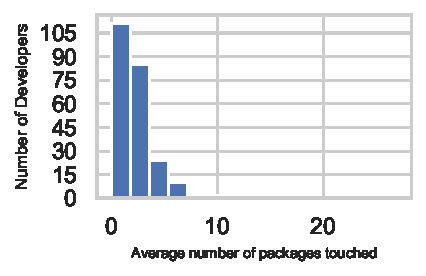
\includegraphics[width=\textwidth]{sections/results/graph/normality_and_homoscedasticity_graph_transient_moderate_2_packages_sample_sustained.packages.touched.commits.pdf}
    \caption{Sustained ($\mu$: 2.38, median:2, mode:1, std:2.61 and max:27)}
    \label{subfig:sections/results/graph/normality_and_homoscedasticity_graph_transient_moderate_2_packages_sample_sustained_packages_touched_commits_pdf}
  \end{subfigure}
\caption{Packages for two commits for  sample A category versus sample B category } 
    \label{fig:codebase_graph_latex_repository_graph_component_time_series_statistical_significance_testpackages2normality_and_homoscedasticity_graph_transient_moderate}
\end{figure}
\clearpage 
\begin{figure}
  \centering 
\vspace{3mm}
  \begin{subfigure}[b]{0.45\textwidth}
    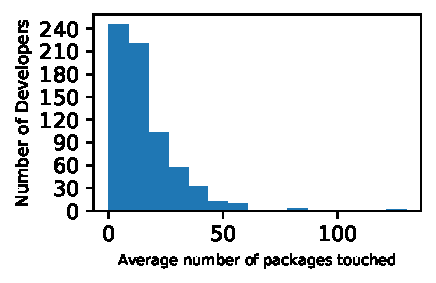
\includegraphics[width=\textwidth]{sections/results/graph/normality_and_homoscedasticity_graph_transient_moderate_5_packages_founder_moderate.packages.touched.commits.pdf}
    \caption{Moderate ($\mu$: 2.59, median:2, mode:1, std:3.06 and max:41)}
    \label{subfig:sections/results/graph/normality_and_homoscedasticity_graph_transient_moderate_5_packages_founder_moderate_packages_touched_commits_pdf}
  \end{subfigure}
  \begin{subfigure}[b]{0.45\textwidth}
    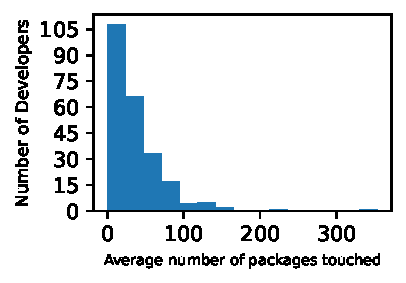
\includegraphics[width=\textwidth]{sections/results/graph/normality_and_homoscedasticity_graph_transient_moderate_5_packages_sample_sustained.packages.touched.commits.pdf}
    \caption{Sustained ($\mu$: 2.38, median:2, mode:1, std:2.61 and max:27)}
    \label{subfig:sections/results/graph/normality_and_homoscedasticity_graph_transient_moderate_5_packages_sample_sustained_packages_touched_commits_pdf}
  \end{subfigure}
\caption{Packages for five commits for  sample A category versus sample B category } 
    \label{fig:codebase_graph_latex_repository_graph_component_time_series_statistical_significance_testpackages5normality_and_homoscedasticity_graph_transient_moderate}
\end{figure}
\clearpage 
\begin{figure}
  \centering 
\vspace{3mm}
  \begin{subfigure}[b]{0.45\textwidth}
    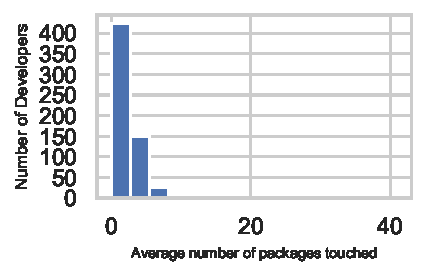
\includegraphics[width=\textwidth]{sections/results/graph/normality_and_homoscedasticity_graph_transient_moderate_10_packages_founder_moderate.packages.touched.commits.pdf}
    \caption{Moderate ($\mu$: 2.55, median:2.0, mode:1, std:2.88 and max:41)}
    \label{subfig:sections/results/graph/normality_and_homoscedasticity_graph_transient_moderate_10_packages_founder_moderate_packages_touched_commits_pdf}
  \end{subfigure}
  \begin{subfigure}[b]{0.45\textwidth}
    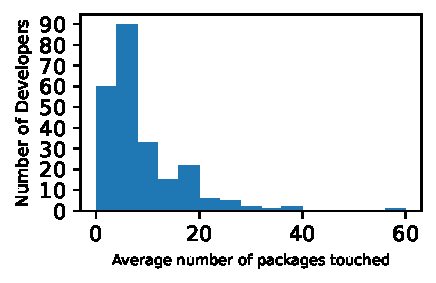
\includegraphics[width=\textwidth]{sections/results/graph/normality_and_homoscedasticity_graph_transient_moderate_10_packages_sample_sustained.packages.touched.commits.pdf}
    \caption{Sustained ($\mu$: 2.38, median:2, mode:1, std:2.61 and max:27)}
    \label{subfig:sections/results/graph/normality_and_homoscedasticity_graph_transient_moderate_10_packages_sample_sustained_packages_touched_commits_pdf}
  \end{subfigure}
\caption{Packages for ten commits for  sample A category versus sample B category } 
    \label{fig:codebase_graph_latex_repository_graph_component_time_series_statistical_significance_testpackages10normality_and_homoscedasticity_graph_transient_moderate}
\end{figure}
\clearpage 
\begin{figure}
  \centering 
    \label{fig:codebase_graph_latex_repository_graph_component_time_series_statistical_significance_testpackages20normality_and_homoscedasticity_graph_transient_moderate}
\end{figure}
\clearpage 
\begin{figure}
  \centering 
\vspace{3mm}
  \begin{subfigure}[b]{0.45\textwidth}
    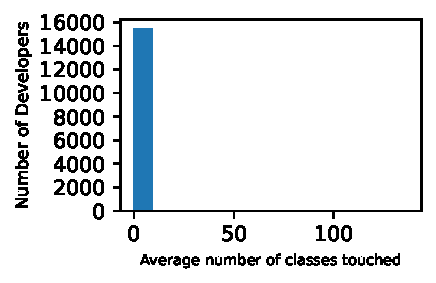
\includegraphics[width=\textwidth]{sections/results/graph/normality_and_homoscedasticity_graph_transient_moderate_1_classes_founder_transient.classes.touched.commits.pdf}
    \caption{Transient ($\mu$: 1.15, median:1.0, mode:1, std:1.95 and max:137)}
    \label{subfig:sections/results/graph/normality_and_homoscedasticity_graph_transient_moderate_1_classes_founder_transient_classes_touched_commits_pdf}
  \end{subfigure}
  \begin{subfigure}[b]{0.45\textwidth}
    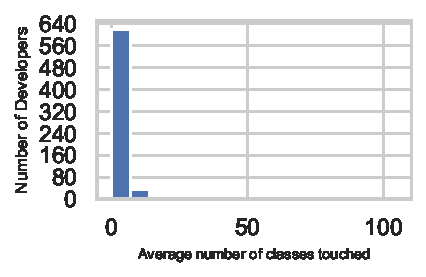
\includegraphics[width=\textwidth]{sections/results/graph/normality_and_homoscedasticity_graph_transient_moderate_1_classes_sample_moderate.classes.touched.commits.pdf}
    \caption{Moderate ($\mu$: 3.24, median:1, mode:1, std:8.5 and max:105)}
    \label{subfig:sections/results/graph/normality_and_homoscedasticity_graph_transient_moderate_1_classes_sample_moderate_classes_touched_commits_pdf}
  \end{subfigure}
\vspace{3mm}
  \begin{subfigure}[b]{0.45\textwidth}
    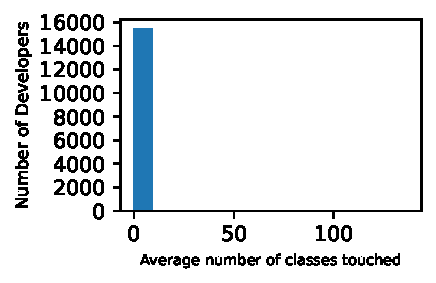
\includegraphics[width=\textwidth]{sections/results/graph/normality_and_homoscedasticity_graph_transient_moderate_1_classes_founder_transient.classes.touched.commits.pdf}
    \caption{Transient ($\mu$: 1.15, median:1.0, mode:1, std:1.95 and max:137)}
    \label{subfig:sections/results/graph/normality_and_homoscedasticity_graph_transient_moderate_1_classes_founder_transient_classes_touched_commits_pdf}
  \end{subfigure}
  \begin{subfigure}[b]{0.45\textwidth}
    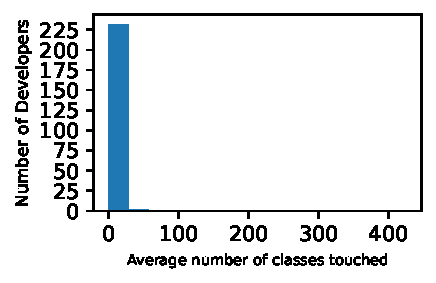
\includegraphics[width=\textwidth]{sections/results/graph/normality_and_homoscedasticity_graph_transient_moderate_1_classes_sample_sustained.classes.touched.commits.pdf}
    \caption{Sustained ($\mu$: 5.19, median:1, mode:1, std:30.1 and max:426)}
    \label{subfig:sections/results/graph/normality_and_homoscedasticity_graph_transient_moderate_1_classes_sample_sustained_classes_touched_commits_pdf}
  \end{subfigure}
\vspace{3mm}
  \begin{subfigure}[b]{0.45\textwidth}
    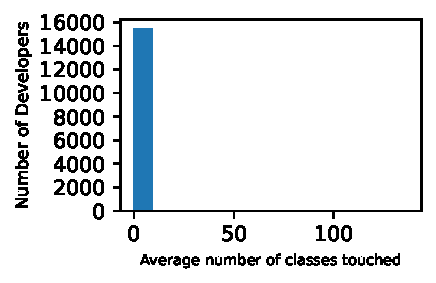
\includegraphics[width=\textwidth]{sections/results/graph/normality_and_homoscedasticity_graph_transient_moderate_1_classes_founder_transient.classes.touched.commits.pdf}
    \caption{Transient ($\mu$: 1.15, median:1.0, mode:1, std:1.95 and max:137)}
    \label{subfig:sections/results/graph/normality_and_homoscedasticity_graph_transient_moderate_1_classes_founder_transient_classes_touched_commits_pdf}
  \end{subfigure}
  \begin{subfigure}[b]{0.45\textwidth}
    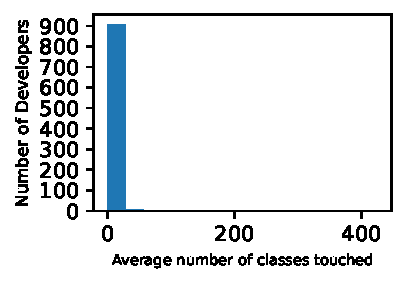
\includegraphics[width=\textwidth]{sections/results/graph/normality_and_homoscedasticity_graph_transient_moderate_1_classes_sample_moderate sustained.classes.touched.commits.pdf}
    \caption{Moderate sustained ($\mu$: 3.74, median:1.0, mode:1, std:16.92 and max:426)}
    \label{subfig:sections/results/graph/normality_and_homoscedasticity_graph_transient_moderate_1_classes_sample_moderate sustained_classes_touched_commits_pdf}
  \end{subfigure}
\vspace{3mm}
  \begin{subfigure}[b]{0.45\textwidth}
    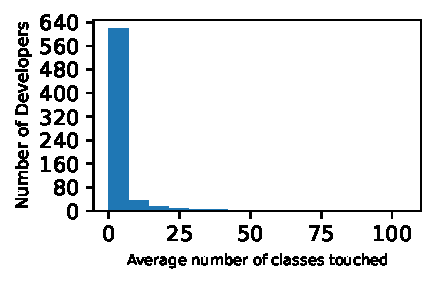
\includegraphics[width=\textwidth]{sections/results/graph/normality_and_homoscedasticity_graph_transient_moderate_1_classes_founder_moderate.classes.touched.commits.pdf}
    \caption{Moderate ($\mu$: 3.24, median:1, mode:1, std:8.5 and max:105)}
    \label{subfig:sections/results/graph/normality_and_homoscedasticity_graph_transient_moderate_1_classes_founder_moderate_classes_touched_commits_pdf}
  \end{subfigure}
  \begin{subfigure}[b]{0.45\textwidth}
    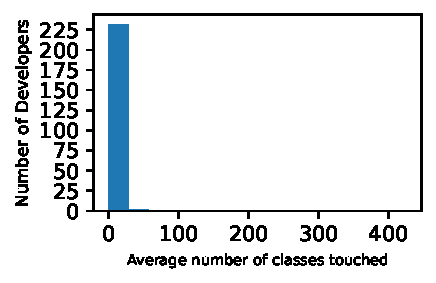
\includegraphics[width=\textwidth]{sections/results/graph/normality_and_homoscedasticity_graph_transient_moderate_1_classes_sample_sustained.classes.touched.commits.pdf}
    \caption{Sustained ($\mu$: 5.19, median:1, mode:1, std:30.1 and max:426)}
    \label{subfig:sections/results/graph/normality_and_homoscedasticity_graph_transient_moderate_1_classes_sample_sustained_classes_touched_commits_pdf}
  \end{subfigure}
\caption{Classes for one commits for  sample A category versus sample B category } 
    \label{fig:codebase_graph_latex_repository_graph_component_time_series_statistical_significance_testclasses1normality_and_homoscedasticity_graph_transient_moderate}
\end{figure}
\clearpage 
\begin{figure}
  \centering 
\vspace{3mm}
  \begin{subfigure}[b]{0.45\textwidth}
    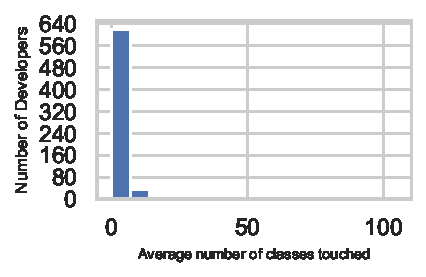
\includegraphics[width=\textwidth]{sections/results/graph/normality_and_homoscedasticity_graph_transient_moderate_2_classes_founder_moderate.classes.touched.commits.pdf}
    \caption{Moderate ($\mu$: 3.24, median:1, mode:1, std:8.5 and max:105)}
    \label{subfig:sections/results/graph/normality_and_homoscedasticity_graph_transient_moderate_2_classes_founder_moderate_classes_touched_commits_pdf}
  \end{subfigure}
  \begin{subfigure}[b]{0.45\textwidth}
    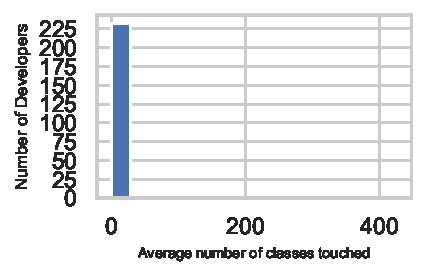
\includegraphics[width=\textwidth]{sections/results/graph/normality_and_homoscedasticity_graph_transient_moderate_2_classes_sample_sustained.classes.touched.commits.pdf}
    \caption{Sustained ($\mu$: 5.19, median:1, mode:1, std:30.1 and max:426)}
    \label{subfig:sections/results/graph/normality_and_homoscedasticity_graph_transient_moderate_2_classes_sample_sustained_classes_touched_commits_pdf}
  \end{subfigure}
\caption{Classes for two commits for  sample A category versus sample B category } 
    \label{fig:codebase_graph_latex_repository_graph_component_time_series_statistical_significance_testclasses2normality_and_homoscedasticity_graph_transient_moderate}
\end{figure}
\clearpage 
\begin{figure}
  \centering 
\vspace{3mm}
  \begin{subfigure}[b]{0.45\textwidth}
    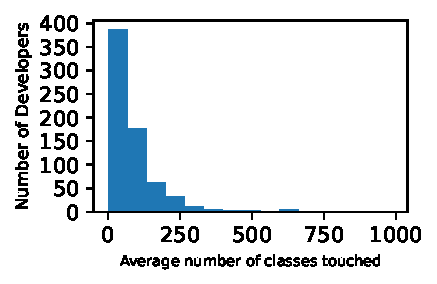
\includegraphics[width=\textwidth]{sections/results/graph/normality_and_homoscedasticity_graph_transient_moderate_5_classes_founder_moderate.classes.touched.commits.pdf}
    \caption{Moderate ($\mu$: 3.24, median:1, mode:1, std:8.5 and max:105)}
    \label{subfig:sections/results/graph/normality_and_homoscedasticity_graph_transient_moderate_5_classes_founder_moderate_classes_touched_commits_pdf}
  \end{subfigure}
  \begin{subfigure}[b]{0.45\textwidth}
    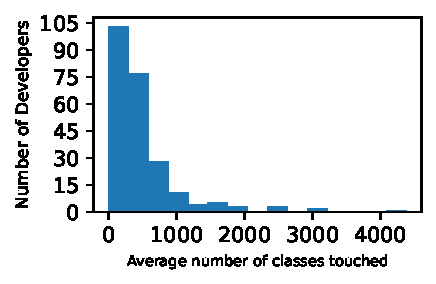
\includegraphics[width=\textwidth]{sections/results/graph/normality_and_homoscedasticity_graph_transient_moderate_5_classes_sample_sustained.classes.touched.commits.pdf}
    \caption{Sustained ($\mu$: 5.19, median:1, mode:1, std:30.1 and max:426)}
    \label{subfig:sections/results/graph/normality_and_homoscedasticity_graph_transient_moderate_5_classes_sample_sustained_classes_touched_commits_pdf}
  \end{subfigure}
\caption{Classes for five commits for  sample A category versus sample B category } 
    \label{fig:codebase_graph_latex_repository_graph_component_time_series_statistical_significance_testclasses5normality_and_homoscedasticity_graph_transient_moderate}
\end{figure}
\clearpage 
\begin{figure}
  \centering 
\vspace{3mm}
  \begin{subfigure}[b]{0.45\textwidth}
    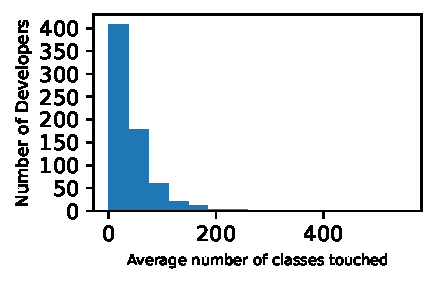
\includegraphics[width=\textwidth]{sections/results/graph/normality_and_homoscedasticity_graph_transient_moderate_10_classes_founder_moderate.classes.touched.commits.pdf}
    \caption{Moderate ($\mu$: 3.3, median:1.0, mode:1, std:8.85 and max:105)}
    \label{subfig:sections/results/graph/normality_and_homoscedasticity_graph_transient_moderate_10_classes_founder_moderate_classes_touched_commits_pdf}
  \end{subfigure}
  \begin{subfigure}[b]{0.45\textwidth}
    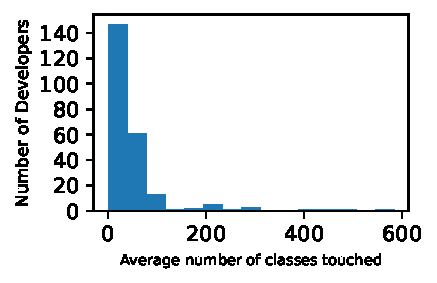
\includegraphics[width=\textwidth]{sections/results/graph/normality_and_homoscedasticity_graph_transient_moderate_10_classes_sample_sustained.classes.touched.commits.pdf}
    \caption{Sustained ($\mu$: 5.19, median:1, mode:1, std:30.1 and max:426)}
    \label{subfig:sections/results/graph/normality_and_homoscedasticity_graph_transient_moderate_10_classes_sample_sustained_classes_touched_commits_pdf}
  \end{subfigure}
\caption{Classes for ten commits for  sample A category versus sample B category } 
    \label{fig:codebase_graph_latex_repository_graph_component_time_series_statistical_significance_testclasses10normality_and_homoscedasticity_graph_transient_moderate}
\end{figure}
\clearpage 
\begin{figure}
  \centering 
    \label{fig:codebase_graph_latex_repository_graph_component_time_series_statistical_significance_testclasses20normality_and_homoscedasticity_graph_transient_moderate}
\end{figure}
\clearpage 
\begin{figure}
  \centering 
\vspace{3mm}
  \begin{subfigure}[b]{0.45\textwidth}
    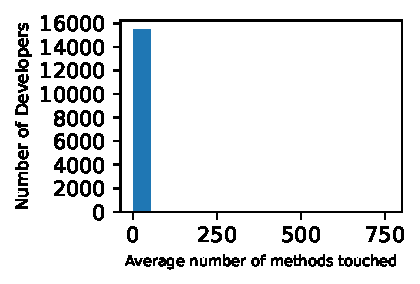
\includegraphics[width=\textwidth]{sections/results/graph/normality_and_homoscedasticity_graph_transient_moderate_1_methods_founder_transient.methods.touched.commits.pdf}
    \caption{Transient ($\mu$: 1.47, median:1.0, mode:1, std:9.29 and max:763)}
    \label{subfig:sections/results/graph/normality_and_homoscedasticity_graph_transient_moderate_1_methods_founder_transient_methods_touched_commits_pdf}
  \end{subfigure}
  \begin{subfigure}[b]{0.45\textwidth}
    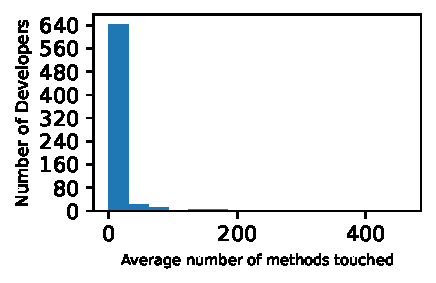
\includegraphics[width=\textwidth]{sections/results/graph/normality_and_homoscedasticity_graph_transient_moderate_1_methods_sample_moderate.methods.touched.commits.pdf}
    \caption{Moderate ($\mu$: 8.9, median:1, mode:1, std:33.8 and max:463)}
    \label{subfig:sections/results/graph/normality_and_homoscedasticity_graph_transient_moderate_1_methods_sample_moderate_methods_touched_commits_pdf}
  \end{subfigure}
\vspace{3mm}
  \begin{subfigure}[b]{0.45\textwidth}
    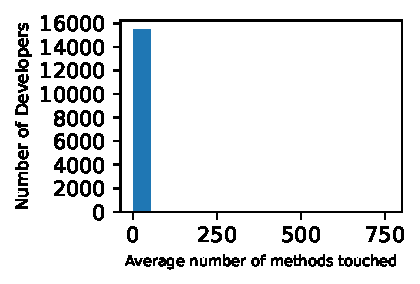
\includegraphics[width=\textwidth]{sections/results/graph/normality_and_homoscedasticity_graph_transient_moderate_1_methods_founder_transient.methods.touched.commits.pdf}
    \caption{Transient ($\mu$: 1.47, median:1.0, mode:1, std:9.29 and max:763)}
    \label{subfig:sections/results/graph/normality_and_homoscedasticity_graph_transient_moderate_1_methods_founder_transient_methods_touched_commits_pdf}
  \end{subfigure}
  \begin{subfigure}[b]{0.45\textwidth}
    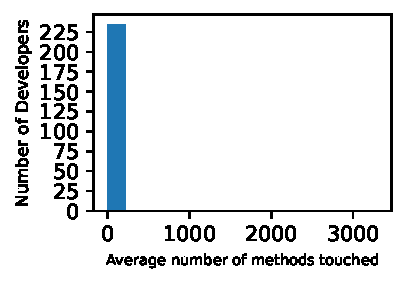
\includegraphics[width=\textwidth]{sections/results/graph/normality_and_homoscedasticity_graph_transient_moderate_1_methods_sample_sustained.methods.touched.commits.pdf}
    \caption{Sustained ($\mu$: 22.14, median:1, mode:1, std:218.06 and max:3301)}
    \label{subfig:sections/results/graph/normality_and_homoscedasticity_graph_transient_moderate_1_methods_sample_sustained_methods_touched_commits_pdf}
  \end{subfigure}
\vspace{3mm}
  \begin{subfigure}[b]{0.45\textwidth}
    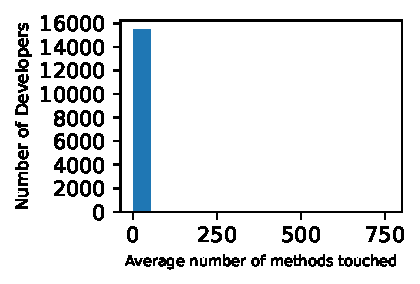
\includegraphics[width=\textwidth]{sections/results/graph/normality_and_homoscedasticity_graph_transient_moderate_1_methods_founder_transient.methods.touched.commits.pdf}
    \caption{Transient ($\mu$: 1.47, median:1.0, mode:1, std:9.29 and max:763)}
    \label{subfig:sections/results/graph/normality_and_homoscedasticity_graph_transient_moderate_1_methods_founder_transient_methods_touched_commits_pdf}
  \end{subfigure}
  \begin{subfigure}[b]{0.45\textwidth}
    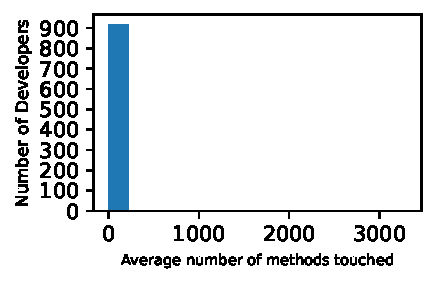
\includegraphics[width=\textwidth]{sections/results/graph/normality_and_homoscedasticity_graph_transient_moderate_1_methods_sample_moderate sustained.methods.touched.commits.pdf}
    \caption{Moderate sustained ($\mu$: 12.3, median:1.0, mode:1, std:114.2 and max:3301)}
    \label{subfig:sections/results/graph/normality_and_homoscedasticity_graph_transient_moderate_1_methods_sample_moderate sustained_methods_touched_commits_pdf}
  \end{subfigure}
\vspace{3mm}
  \begin{subfigure}[b]{0.45\textwidth}
    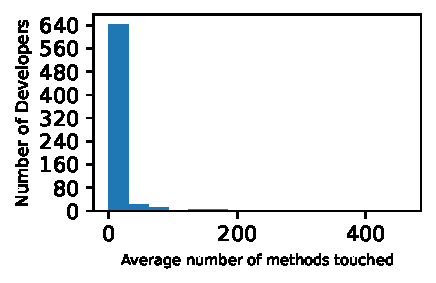
\includegraphics[width=\textwidth]{sections/results/graph/normality_and_homoscedasticity_graph_transient_moderate_1_methods_founder_moderate.methods.touched.commits.pdf}
    \caption{Moderate ($\mu$: 8.9, median:1, mode:1, std:33.8 and max:463)}
    \label{subfig:sections/results/graph/normality_and_homoscedasticity_graph_transient_moderate_1_methods_founder_moderate_methods_touched_commits_pdf}
  \end{subfigure}
  \begin{subfigure}[b]{0.45\textwidth}
    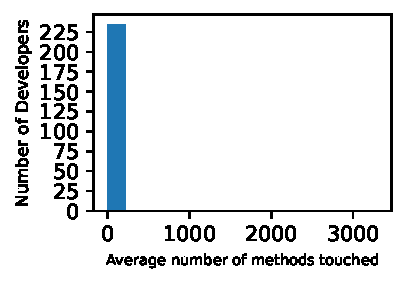
\includegraphics[width=\textwidth]{sections/results/graph/normality_and_homoscedasticity_graph_transient_moderate_1_methods_sample_sustained.methods.touched.commits.pdf}
    \caption{Sustained ($\mu$: 22.14, median:1, mode:1, std:218.06 and max:3301)}
    \label{subfig:sections/results/graph/normality_and_homoscedasticity_graph_transient_moderate_1_methods_sample_sustained_methods_touched_commits_pdf}
  \end{subfigure}
\caption{Methods for one commits for  sample A category versus sample B category } 
    \label{fig:codebase_graph_latex_repository_graph_component_time_series_statistical_significance_testmethods1normality_and_homoscedasticity_graph_transient_moderate}
\end{figure}
\clearpage 
\begin{figure}
  \centering 
\vspace{3mm}
  \begin{subfigure}[b]{0.45\textwidth}
    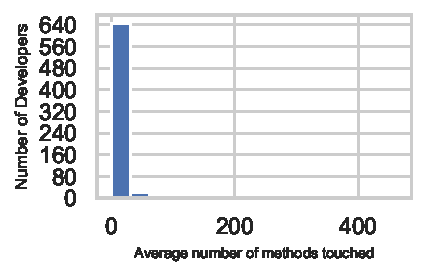
\includegraphics[width=\textwidth]{sections/results/graph/normality_and_homoscedasticity_graph_transient_moderate_2_methods_founder_moderate.methods.touched.commits.pdf}
    \caption{Moderate ($\mu$: 8.9, median:1, mode:1, std:33.8 and max:463)}
    \label{subfig:sections/results/graph/normality_and_homoscedasticity_graph_transient_moderate_2_methods_founder_moderate_methods_touched_commits_pdf}
  \end{subfigure}
  \begin{subfigure}[b]{0.45\textwidth}
    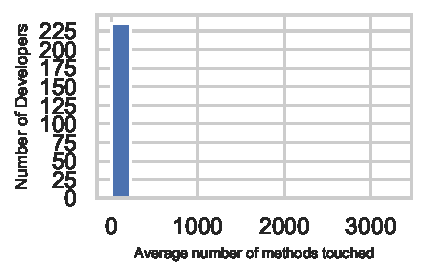
\includegraphics[width=\textwidth]{sections/results/graph/normality_and_homoscedasticity_graph_transient_moderate_2_methods_sample_sustained.methods.touched.commits.pdf}
    \caption{Sustained ($\mu$: 22.14, median:1, mode:1, std:218.06 and max:3301)}
    \label{subfig:sections/results/graph/normality_and_homoscedasticity_graph_transient_moderate_2_methods_sample_sustained_methods_touched_commits_pdf}
  \end{subfigure}
\caption{Methods for two commits for  sample A category versus sample B category } 
    \label{fig:codebase_graph_latex_repository_graph_component_time_series_statistical_significance_testmethods2normality_and_homoscedasticity_graph_transient_moderate}
\end{figure}
\clearpage 
\begin{figure}
  \centering 
\vspace{3mm}
  \begin{subfigure}[b]{0.45\textwidth}
    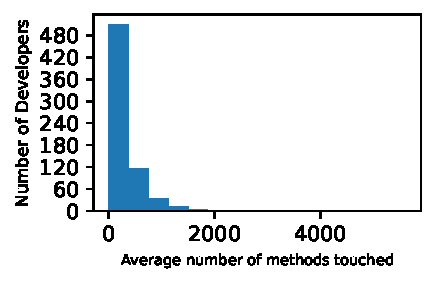
\includegraphics[width=\textwidth]{sections/results/graph/normality_and_homoscedasticity_graph_transient_moderate_5_methods_founder_moderate.methods.touched.commits.pdf}
    \caption{Moderate ($\mu$: 8.9, median:1, mode:1, std:33.8 and max:463)}
    \label{subfig:sections/results/graph/normality_and_homoscedasticity_graph_transient_moderate_5_methods_founder_moderate_methods_touched_commits_pdf}
  \end{subfigure}
  \begin{subfigure}[b]{0.45\textwidth}
    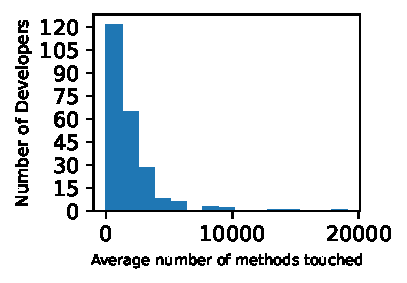
\includegraphics[width=\textwidth]{sections/results/graph/normality_and_homoscedasticity_graph_transient_moderate_5_methods_sample_sustained.methods.touched.commits.pdf}
    \caption{Sustained ($\mu$: 22.14, median:1, mode:1, std:218.06 and max:3301)}
    \label{subfig:sections/results/graph/normality_and_homoscedasticity_graph_transient_moderate_5_methods_sample_sustained_methods_touched_commits_pdf}
  \end{subfigure}
\caption{Methods for five commits for  sample A category versus sample B category } 
    \label{fig:codebase_graph_latex_repository_graph_component_time_series_statistical_significance_testmethods5normality_and_homoscedasticity_graph_transient_moderate}
\end{figure}
\clearpage 
\begin{figure}
  \centering 
\vspace{3mm}
  \begin{subfigure}[b]{0.45\textwidth}
    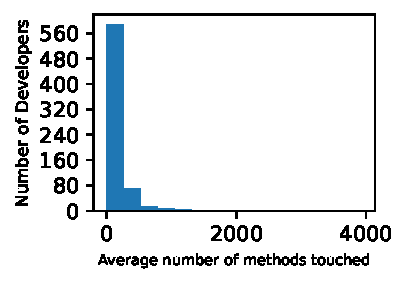
\includegraphics[width=\textwidth]{sections/results/graph/normality_and_homoscedasticity_graph_transient_moderate_10_methods_founder_moderate.methods.touched.commits.pdf}
    \caption{Moderate ($\mu$: 8.92, median:1.0, mode:1, std:34.39 and max:463)}
    \label{subfig:sections/results/graph/normality_and_homoscedasticity_graph_transient_moderate_10_methods_founder_moderate_methods_touched_commits_pdf}
  \end{subfigure}
  \begin{subfigure}[b]{0.45\textwidth}
    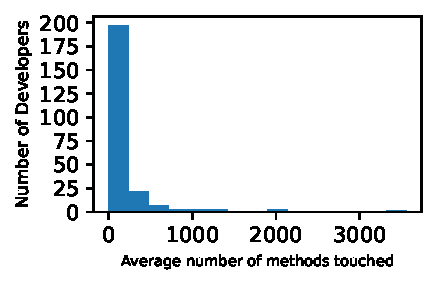
\includegraphics[width=\textwidth]{sections/results/graph/normality_and_homoscedasticity_graph_transient_moderate_10_methods_sample_sustained.methods.touched.commits.pdf}
    \caption{Sustained ($\mu$: 22.14, median:1, mode:1, std:218.06 and max:3301)}
    \label{subfig:sections/results/graph/normality_and_homoscedasticity_graph_transient_moderate_10_methods_sample_sustained_methods_touched_commits_pdf}
  \end{subfigure}
\caption{Methods for ten commits for  sample A category versus sample B category } 
    \label{fig:codebase_graph_latex_repository_graph_component_time_series_statistical_significance_testmethods10normality_and_homoscedasticity_graph_transient_moderate}
\end{figure}
\clearpage 
\begin{figure}
  \centering 
    \label{fig:codebase_graph_latex_repository_graph_component_time_series_statistical_significance_testmethods20normality_and_homoscedasticity_graph_transient_moderate}
\end{figure}
\clearpage 
